\cotefile{157-5}
\scanpage{513}
\mspage{425}
% B01
4.15. \uline{Catégorie accessible sur une autre}.

% B02
\uline{Proposition} 4.15.1. Soit $f:E\unsure{\relbar|\longrightarrow} C$ un foncteur, avec $C$ \deleted{\unsure{essentiellement}} petite, \deleted{$E$ et $f$ \unsure{satisfaisant|satisfont} à la condition \unsure{la|H}.} On suppose de plus satisfaite la condition $H$ (p. 409), qu'on explicite \unsure{ici} sous la forme équivalente $H'$)

% B03
$H\unsure{'|^{*}}1)$ Pour tout $s\in\mathrm{Ob}\,C$, $E_s$ est accessible

% B04
$H'\deleted{\unsure{2}}3)$ Pour tt $\lambda\in\deleted{\unsure{\mathrm{Ob}}}\mathrm{Fl}\,C$, $\lambda:s\to t$, et pour tout $x_0\in\mathrm{Ob}\,E_s$, le foncteur
% B05
\[x_1\longrightarrow\mathrm{Hom}_{\lambda}(x_0,x_1):\quad E_t\unsure{\relbar|\longrightarrow}(\mathrm{Ens})\]
% B06
est accessible

% B07
\margin{\figure{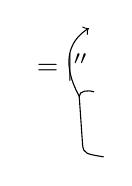
\begin{tikzpicture}[x=.27cm,y=.27cm]\node at (-.79,4.2) {$\unsure{=|''}$};\draw (1.15,0) .. controls (.35,.13) and (.2,.15) .. (.16,.55) -- (0,2.85) .. controls (0,3.12) and (.44,3.15) .. (.7,3.06);\draw[->] (0,2.85) .. controls (-1,4.7) and (-.25,5.6) .. (.45,6.05);\end{tikzpicture}}}

% B08
$H'\deleted{\unsure{3}}2)$ Pour tt $\lambda\in\mathrm{Fl}\,C$, $\lambda:s\to t$, existe un cardinal infini $\pi_\lambda$ tel que pour tt $x_1\in\mathrm{Ob}\,E_t$, le foncteur
% B09
\[x_0\longmapsto\mathrm{Hom}_{\lambda}(x_0,x_1):\quad E_s\longrightarrow(\mathrm{Ens})^\circ\]
% B10
est $\pi_\lambda$-accessible\deleted{\unsure{s}} ($E_s$ satisfaisant de plus \unsure{:|à} $L_{\pi_\lambda}$).

% B11
Alors \deleted{$E$ est accessible, et $f$ accessible \unsure{(pour} \inserted{\deleted{\unsure{satisfait},}} \illegible{3} \unsure{hypothèses|hypothèse}), \unsure{de façon plus précise},} les foncteurs d'inclusion $i_s:E_s\longrightarrow E$ sont accessibles. De plus, si $C$ est ``sans projecteurs'' (i.e si tout endom. $p$ d'un \unsure{objet} $s$ de $C$, tel que $p^2=p$, est l'identité), alors $E$ est accessible, et $p:E\to C$ est accessible.

% B12
Cela résulte des résultats plus précis

% B13
\deleted{\uline{Corollaire} 4.15.2. \unsure{a)} Soit \inserted{$s\in\mathrm{Ob}\,C$ et} $\pi_0$ un cardinal \deleted{\unsure{majorant les} \illegible{2} $E_s$ tel que : $\pi_0$} \inserted{\unsure{$E$ et $f$ satisfont}} tel que \unsure{a)} $\pi_0$ majore les $\pi_\lambda$ intervenant dans $H'3)$, pour $\lambda:s\to t$ (\unsure{flèche} de source \unsure{s})}

% archive sheet number: 512
\scanpage{514}
\mspage{426}
\deleted{
% B01
Alors \deleted{\unsure{les}} $i_s:E_s\unsure{\relbar|\longrightarrow}E$ satisfait \unsure{:|à} $L_{\pi_0}$

% B02
[En particulier, si $\pi_0$ est choisi de façon que $\pi_0$ majore tous les $\pi_\lambda$ ($\lambda\in\mathrm{Fl}\,C$), \deleted{alors} (c'est possible car $\mathrm{Fl}\,C$ est petit) alors $\forall s\in\mathrm{Ob}\,\unsure{S|C}$, $i_s:E_s\relbar E$ satisfait $L_{\pi_0}$.]

% B03
% margin note written sideways
\margin{$1)$ $\pi_0\geq\underset{\lambda\in\mathrm{Fl}\,C}{\mathrm{Sup}}\ \pi_\lambda$\\ $2)$ $\pi_1\geq\sup(\pi_0,\mathrm{card}\,C,\underset{s\in\mathrm{Ob}\,C}{\mathrm{Sup}}(\mathrm{card\,red}\,E_{s\pi_0})$.}

% B04
b) \inserted{Supposons $C$ \uline{sans projecteurs}.} \deleted{\unsure{Si} \unsure{tel} \unsure{quel} \unsure{que} \illegible{2} $\pi_0$ \unsure{sup} \illegible{1}} \inserted{$\pi_0\geq\underset{\lambda\in\mathrm{Fl}\,C}{\mathrm{Sup}}\pi_\lambda$,} \unsure{Soit|soient} $\pi_0,\pi_1$ tels que \deleted{\unsure{et soit} $\pi_1$ un cardinal $\unsure{\mathrm{card}\,C},\underset{s\in\mathrm{Ob}\,C}{\mathrm{Sup}}(\mathrm{card}\ \unsure{E_{s\pi_0}})$ \unsure{Sup} \illegible{2} $\mathrm{card}\,E_{s\pi_0}$} tel que \deleted{\illegible{2} $(\pi_0,\mathrm{card\,red}\,E_{s\pi_0})$, \unsure{satisfait au cardinal} $L_{\pi_1}$} Alors $E$ satisfait à $L_{\pi_1}$, et si $\pi$ est tel que \deleted{\illegible{1}} $\pi^{\pi_0}=\pi\geq\pi_1$, Alors
% B05
\[i_s(E_{s\pi})\subset E_\pi.\]

% B06
c) \inserted{\unsure{Sous les} hypothèses sur $C,\pi_0,\pi_1$ de \unsure{b)|b},} Pour tout cardinal $\pi$, soit $E(\pi)$ la sous-catégorie pleine de $E$ \deleted{\unsure{formée des}} telle que
% B07
\[\mathrm{Ob}\,E(\pi)=\bigcup_{s\in\mathrm{Ob}\,C}\mathrm{Ob}\,E_{s\pi}.\]

% B08
\deleted{Soit $\pi_0$ tel que $\pi_0\geq\underset{\lambda\in\mathrm{Fl}\,C}{\mathrm{Sup}}\pi_\lambda$, et $\pi_1\geq\pi_0$ un cardinal tel que $\pi_1\geq\underset{\deleted{\unsure{\lambda\in\mathrm{Fl}\,C|\mathrm{Fl}\,C}}\,s\in\mathrm{Ob}\,C}{\mathrm{Sup}}(\mathrm{card\,red}\,E_{s\pi_0})$, et que $E$ satisfasse $L_{\pi_1}$.}

% B09
Soit $\pi$ un cardinal tel que $\pi^{\pi_0}=\pi\geq\unsure{\pi_1|I_1}$, \deleted{et tel que $E$ satisfasse à $L_\pi$} Alors
% B10
\[E(\pi)\subset E_\pi,\]
% B11
d'où un foncteur pleinement fidèle ($E$ satisfaisant \unsure{:|à} $L_\pi$)
% B12
\[\mathrm{Ind}_\pi E(\pi)\longrightarrow E,\]
% B13
et ce foncteur est une équivalence (donc $E$ est accessible).

}
% archive sheet number: 513
\scanpage{515}
\mspage{426}
% B01
\uline{Corollaire} 4.15.2. Les hypothèses sur $f:E\unsure{\relbar|\longrightarrow}C$ sont celles de 4.15.1 ($C$ petite, et $f$ satisfait $H'=H1)2)3)$).

% B02
% slanted
\margin{\inserted{Pour a) et b),} On n'utilise que $H1$ et $H2$, à l'exclusion de $H3$.}

% B03
a) Soit $s\in\mathrm{Ob}\,C$ et soit $\pi_1$ un cardinal infini tel que pour tt $\lambda:s\to t$ (flèche de $C$ de source $t$), on ait $\pi_1\geq\pi_\lambda$ (où $\pi_\lambda$ est défini dans l'énoncé de $H2$). Alors le foncteur $i_s:E_s\longrightarrow E$ \deleted{satisfait} est $\pi_1$-accessible.

% B04
b) \inserted{On suppose $C$ \uline{sans projecteurs}.} Soit $\pi_{\deleted{\unsure{0}}1}$ un cardinal \deleted{\unsure{infini tel que,} 1, les catégories $E_s$ ($s\in\mathrm{Ob}\,C$) satisfassent $L_{\pi_1}$ (existe car : $H1)$ et au fait que $C$ ou $\mathrm{Ob}\,C$ petit)), et tel que $\pi_1\geq\mathrm{card}\,\deleted{\unsure{\mathrm{Ob}}}C$.} \inserted{$\geq\mathrm{Sup}(\underset{\lambda}{\mathrm{Sup}}\pi_\lambda,\mathrm{card}\,C)$} Alors $E$ satisfait $L_{\pi_1}$, et $f:E\to C$ est $\pi$-accessible.

% B05
c) \deleted{Soit $\pi_0$ un \unsure{cardinal}} \inserted{Supposons} que $C$ soit sans projecteurs. (p. ex une catégorie ``rigide'', p. ex. une catégorie \inserted{pré}ordonnée). Soient $\pi_0,\pi_1$ des cardinaux tels que

% B06
\textcircled{\scriptsize $1^\circ$} \deleted{$\pi_0\geq\unsure{\sup}$ \unsure{que}} $\forall s\in\mathrm{Ob}\,C$, $\pi_0$ est \uline{utile pour} $E_s$ (\inserted{un tel $\pi_0$} existe grâce à $H1)$ et au fait que $C$ \deleted{\unsure{est un}} $\mathrm{Ob}\,C$ petit).

% B07
\textcircled{\scriptsize $2^\circ$} $\pi_1\geq\mathrm{Sup}(\pi_0,\inserted{\mathrm{card}\,C,}\underset{\lambda\in\mathrm{Fl}\,C}{\mathrm{Sup}}\pi_\lambda,\underset{s\in\mathrm{Ob}\,C}{\mathrm{Sup}}\underline{\mathrm{card\,red}}\ E_{s\pi_0})$.

% B08
\textcircled{\scriptsize $3^\circ$} $\forall\lambda\in\mathrm{Fl}\,C$, et $x_0\in\mathrm{Ob}\,E_{s,\pi_0}$, le foncteur $\unsure{H_\lambda|h_\lambda|h} (x_0)$ de $H3$ \inserted{$x_1\longmapsto\mathrm{Hom}_{\lambda}(x_0,x_1): E_t\longrightarrow\mathrm{Ens}$ est $\pi_1$-\uline{accessible}.}
% slanted

% B09
Soit $\pi$ \deleted{\unsure{$\geq\pi_1$}} un cardinal tel que $\pi^{\pi_0}=\pi\geq\pi_1$. Alors Par b) $E$ satisfait $L_{\pi_1}$ donc $L_\pi$, et $f:E\to C$ est $\pi_1$-accessible\deleted{\unsure{ment}}, De plus
% B10
\[i_s(E_{s\pi})\subset E_\pi,\]
% B11
\deleted{d'où} ou encore \deleted{et \unsure{$E_\pi$} d'où un foncteur pl. fid ($E_\pi$ satisfaisant à $L_{\pi_1}$, et a fortiori à $L_\pi$, grâce à b)} \inserted{(cf)}
% B12
\[E(\pi)\subset E_\pi,\]
% B13
où $E(\pi)$ est la sous-catégorie pl. de $E$ \deleted{formée des} telle que
% B14
\[\mathrm{Ob}\,E(\pi)=\bigcup_{s\in\mathrm{Ob}\,C}\mathrm{Ob}(E_{s\pi}).\]

% B15
Comme $E_\pi$ satisfait $L_{\pi_1}$ par b), donc a fortiori $L_\pi$, on a donc en ce cas un foncteur \uline{pl fid.}
% B16
\[\mathrm{Ind}_{\pi}(E_{s\pi})\xrightarrow{\approx}E_{\deleted{\unsure{s|\pi}}},\]
% B17
et ce foncteur est une équivalence de catégories (donc $E$ est accessible).

% B18
d) En fait, sous les hyp. de c) sur $C,\pi_0,\unsure{\pi_\lambda|\pi_1},\pi$, on a $E(\pi)=E_\pi$ ! (\unsure{ou|non} seulement $E(\pi)\subset E_\pi$)

% archive sheet number: 514
\scanpage{516}
\mspage{427}
% B01
\uline{Dém} \inserted{de 4.15.1 et 4.15.2.} Il est clair que \deleted{\unsure{8}}4.15.1 est contenu dans 4.15.2 a) et c). Nous allons donc prouver 4.15.2.

% B02
a) Soit $(x_i)_{i\in I}$ un système inductif dans $E_s$, avec $I$ grd devant $\pi_1$, et $x$ sa limite ind. dans $E_s$ \inserted{(qui existe, car $E_s$ satisfait à $L_{\pi_\lambda}$ donc \unsure{à|:} $L_{\pi_0}$)}. Il faut prouver que c'est une limite dans $E$, donc que pour tt $y\in\mathrm{Ob}\,E$, la flèche canonique
% B03
{\csname tagsleft@true\endcsname
\[\deleted{\unsure{\lim}}\,\mathrm{Hom}_E(\unsure{x|y},y)\unsure{\relbar|\longrightarrow}\varprojlim_I\mathrm{Hom}_E(x_i,y)\tag*{\unsure{(a)|(*)}}\]}
% B04
est un iso. Or $\mathrm{Hom}_E(x,y)$ et les $\mathrm{Hom}_E(x_i,y)$ sont des objets de $\mathrm{Ens}_{/\mathrm{Hom}_C(s,t)}$, où $s=f(x)$, $t=f(y)$, et les flèches de transition sont des flèches de $\mathrm{Ens}_{/\mathrm{Hom}_C(s,t)}$. Cela montre que la bijectivité de \unsure{(a)|(*)} revient à \unsure{celles|celle} des
% B05
{\csname tagsleft@true\endcsname
\[\mathrm{Hom}_\lambda(x,y)\relbar\varprojlim_I\mathrm{Hom}_\lambda(x_i,y)\tag*{\unsure{(a)|(* )}}\]}
% B06
pour tout $\lambda\in\mathrm{Hom}_C(x,y)$. Pour $\lambda$ fixé, et $y$ fixé dans $\mathrm{Ob}\,E_t$, la bijectivité en \unsure{qs|qn}, pour tout système inductif grd devant $\pi_1$ dans $E_s$, de limite $x$, signifie que le foncteur
% B07
\[x\longmapsto\mathrm{Hom}_\lambda(x,y):\quad\deleted{\unsure{E| \mathrm{Ens}}}E_s\relbar(\mathrm{Ens})^\circ\]
% B08
est $\pi_{\unsure{0|1}}$-accessible. Or c'est bien le cas, par hypothèse sur $\pi_1$, quel que soit la flèche \deleted{\unsure{$\lambda$ de sou}} $\lambda:s\to t$ de source $s$, et quel que soit $y\in\mathrm{Ob}\,E_t$.

% archive sheet number: 515
\scanpage{517}
\mspage{428}
% B01
\deleted{b) Si $\pi_0,\pi_1,\pi$ sont choisis comme indiqué, il faut voir que $i_s(E_{s\pi})\subset E_\pi$, i.e que tt $x\in\mathrm{Ob}(E_{s\pi})$ est dans $E_\pi$. Il faut donc prouver que pour tt système inductif $(y_i)_{i\in I}$ grd devant $\pi$, \inserted{de limite $y$ dans $E$, (qui existe par hypothèse sur $\pi_1$ et $\pi\geq\pi_1$),} la flèche canonique
{\csname tagsleft@true\endcsname
\[\varinjlim_I\mathrm{Hom}_E(x,y_i)\longrightarrow\mathrm{Hom}_E(x,y)\tag*{\unsure{(**)|($w$)}}\]}
est bijective.}

% B02
b) Soit $(x_i)_{i\in I}$ un système inductif grd devant $\pi_1$, et $(s_i)_{\unsure{j|i}\in I}$ l'image de ce système dans $C$. \deleted{On verra plus \unsure{b|bas}} Nous prouvons plus bas le

% B03
\uline{Lemme} 4.15.3. Soit $C$ une catégorie, \inserted{$\pi$ un cardinal} tels que $\mathrm{card}\,C\leq\pi$, et que $C$ soit sans projecteurs.

% B04
% slanted
\margin{Cf démonstration page 452.}
% B05
Alors pour tout système inductif $(s_i)_{i\in I}$ grd devant $\pi$ dans $C$, existe une partie cofinale \deleted{de} $J$ de $I$ telle que \deleted{les morphismes de \unsure{de} transition du} le système induit $(s_i)_{i\in J}$ soit \uline{constant}, i.e. tel que les $s_i$ soient égaux à un $s\in C$, et que les morphismes de transition soient \deleted{\unsure{l'identité de}} \inserted{tous} \unsure{égaux|identiques} à $\mathrm{id}_s$.

% B06
% slanted
\margin{Sous \unsure{réserve|réserves} de la validité du \unsure{corollaire|coroll.} de 4.8.13. Mais c'est à présent établi, sous une \unsure{forme|hyp.} \unsure{suffisante|plus suffisante|moins restrictive}, \unsure{cf.} \unsure{4.15.6 a) 1°]|4.15.6 a) 1°|4.15.6 a)}}

% B07
Mais Attention, on s'appuie pour prouver 4.15.3 sur \inserted{le th.} 4.8.13 (pages 212--216), que je n'ai tjrs pas prouvé ! Dans le cas où $C$ est rigide (i.e. $\mathrm{End}_C(s)=\{\mathrm{id}_s\}\quad\forall s\in\mathrm{Ob}\,\unsure{E|C}$), la démonstration est cependant immédiate, cf plus bas.

% archive sheet number: 516
\scanpage{518}
\mspage{429}
% B01
Pour prouver que $x=\underset I{\unsure{\underline{\lim}|\varinjlim}}\,x_i$ existe dans $E$, et commute à $f$, on peut remplacer $I$ par une sous-catégorie cofinale. Cela nous ramène, grâce au lemme, au cas où $(s_i)_{i\in I}$ est constant, donc au cas où le système inductif provient d'un système inductif dans une catégorie fibre \inserted{$E_s$}. Mais par a), on sait que sa limite $x$ dans $E_s$ est une limite dans $E$, \unsure{d'où|\deleted{d'où}} l'existence de cette dernière, et la commutation à $f$, puisque $\underset i{\underline{\lim}}\,\deleted{\unsure{f}}(s_i)=s$ ($\underline{\lim}$ d'un syst. inductif filtrant constant).

% B02
c) Il faut prouver que si $x\in\mathrm{Ob}\,E_s$ est $\pi$-accessible \deleted{\unsure{il est}} dans $E_s$, il l'est dans $E$, i.e. que pour tt syst. inductif $(y_i)_{i\in I}$ grd devant $\pi$, la flèche canonique
% B03
{\csname tagsleft@true\endcsname
\[\varinjlim_i\mathrm{Hom}(x,y_i)\longrightarrow\mathrm{Hom}(x,y)\tag*{(**)}\]}
% B04
est bijective. Or \unsure{comme|\deleted{le} comme} \inserted{par $2^\circ$)} $\pi\geq\pi_1\geq\mathrm{Sup}(\mathrm{card}\,\unsure{E|C},\underset{\lambda}{\mathrm{Sup}}\pi_\lambda)$, il résulte encore du lemme que, quitte à remplacer $I$ par une ss-cat. cofinale, \unsure{OPS|OP S} que le système inductif $(y_i)_{i\in I}$ provient d'un système dans \deleted{\unsure{E}} une catégorie fibre $E_t$, et que $y$ est sa $\unsure{\underset{\longrightarrow}{\mathrm{limite}}|\varinjlim^{i}|\varinjlim}$ dans $E_t$.

% B05
\deleted{\unsure{On a vu de}} \inserted{Mais alors} les ens $\mathrm{Hom}(x,y)$ et $\mathrm{Hom}(x,y_i)$, et les \deleted{\unsure{applications}} applications de transition entre celles-ci, sont encore dans $\unsure{\overline{\mathrm E}\mathrm{ns}|\mathrm{Ens}}_{/\mathrm{Hom}(s,t)}$, et on est ramené

% archive sheet number: 517
\scanpage{519}
\mspage{430}
% B01
à prouver que pour tout $\lambda:s\relbar t$, la flèche
% B02
\[\underset i{\unsure{\underline{\lim}|\varinjlim}}\,\mathrm{Hom}_{\lambda}(x,y_i)\longrightarrow\mathrm{Hom}_{\lambda}(x,y)\]
% B03
est bijective. Pour \unsure{$a$|$x$} \inserted{et $\lambda$} \deleted{\unsure{$a$|$x$}} fixés, et des syst. inductifs \unsure{variables|arbitraires} dans $E_t$, grd devant $\pi$, cela signifie que le foncteur
% B04
\[H_\lambda(x)=(y\longmapsto\mathrm{Hom}_\lambda(x,y)):\quad E_t\unsure{\relbar|\longrightarrow}\mathrm{Ens}\]
% B05
est $\pi$-accessible, et ceci quel que soit
% B06
\[x\in\mathrm{Ob}\,E_{s\pi}.\]

% B07
Or c'est le cas si $x\in\mathrm{Ob}\,E_{s\pi_0}$, en vertu de l'hyp. $3^\circ$) (\deleted{\unsure{car que}} alors $H_\lambda(x)$ est $\pi_1$-accessible, et a fortiori $\pi$-accessible). Il faut \deleted{\unsure{prouver}} passer de là au cas où $x\in\mathrm{Ob}\,E_{s\pi}$. Or comme $\pi_0$ est utile pour $E_s$ par $1^\circ$, on a
% B08
\[x=\varinjlim_{j\in J}x_j\qquad\left|\begin{aligned}&x_j\in\mathrm{Ob}\,E_{s\pi_0}\\&J\ \text{grd devant }\pi_0,\end{aligned}\right.\]
% B09
et comme \inserted{par $2^\circ$)} \inserted{on a} $\pi^{\pi_0}=\pi\geq\pi_1\geq\deleted{\unsure{\mathrm{card}}}\mathrm{Sup}(\pi_0,\mathrm{card\,red}\ E_{s\pi_0})$, on en conclut qu'on peut prendre $J$ de sorte que
% B10
\[\mathrm{card}\,J\leq\pi.\]

% B11
D'autre part, en vertu de $\pi\geq\pi_1\geq\pi_\lambda$, le foncteur
% B12
\[\left|\begin{aligned}x_0&\longmapsto H_\lambda(x_0)\\ E_s&\longrightarrow(\underline{\mathrm{Hom}}(E_t,\mathrm{Ens}))^\circ\end{aligned}\right.\]
% B13
est $\pi_0$-accessible, donc on a
% B14
\[H_\lambda(x_0)\simeq\varprojlim_{j\in J}H_\lambda(x_j).\]

% archive sheet number: 518
\scanpage{520}
\mspage{431}
% B01
\unsure{Comme} $x_j\in\mathrm{Ob}\,E_{s\pi_0}$, $H(x_j)$ est un foncteur $\pi_{\unsure{4|1|{}}}$-accessible, \deleted{et} comme $\mathrm{card}\,J\leq\unsure{\Pi|\pi}$, la $\varprojlim_{j\unsure{\in|{\leftarrow}}J}H_\lambda(\unsure{\cdot|{}}x_j)$ est aussi $\pi$-accessible (cf SGA 4 I 9.8).

% B02
Ainsi on a prouvé $E_{s\pi}\subset E(\pi)$ pour tout $s\in\mathrm{Ob}\,C$, i.e. l'inclusion
% B03
\[E(\pi)\subset E_\pi,\]
% B04
d'où le foncteur pl. fidèle
% B05
{\csname tagsleft@true\endcsname
\[\mathrm{Ind}_\pi(E(\pi))\longrightarrow E,\tag*{$(\unsure{\alpha|a})$}\]}
% B06
comme $E$ satisfait à $L_{\unsure{\pi|{}}}$. Il reste à prouver que c'est ess. surjectif. Mais si $x\in\mathrm{Ob}\,E$, $s=f(\unsure{s|x})$, on a $x\in\mathrm{Ob}\,E_s$ et comme $\pi_0$ est utile pour $E_s$ \deleted{donc} \inserted{par $1^\circ$)}, et $\pi^{\pi_0}=\pi>\pi_0$, $\pi$ est également utile pour $\pi$, donc on a
% B07
\[x=\varinjlim_I x_i\quad\left|\begin{aligned}&\text{\uline{dans} }E_s\\&\text{les }x_i\in E_{s\pi_{\unsure{0|{}}}}\subset E(\pi)\\&I\ \text{grd devant }\pi,\end{aligned}\right.\]
% B08
et d'après a) (comme $\pi\geq\pi_1\geq\underset{\lambda\in\mathrm{Fl}}{\mathrm{Sup}}\,\pi_\lambda$) $x$ est aussi limite des $x_i$ dans $E$, donc il est dans \deleted{\unsure{$E$|$\mathrm{Ess}$}} l'image ess. de \unsure{($\alpha$)|($a$)}.

% B09
d) Reste à prouver que l'on a $E_\pi\subset E(\pi)$. Mais on sait (par 4.8.\ \unsure{. --|--}), \deleted{que $E_\pi=$} comme $E\cong\mathrm{Ind}_\pi(E(\pi))$, que $E_\pi=E(\pi)^{\unsure{\natural|\sharp}}$, i.e. \inserted{que pour $x\in\mathrm{Ob}\,E_\pi$,} $\exists y\in E(\pi)$ et un projecteur $p$ dans $y$, tel que $x$ soit iso. à l'image de $p$ dans $E$.

% B10
Or $f(p)$ est un projecteur dans $f(y)=s$, donc par hyp. sur $C$ $f(p)\unsure{\simeq|=}\mathrm{id}_s$ i.e. $p$ est un projecteur dans $E_s$. Comme \deleted{$E_{s\pi}$ est \unsure{fermée}} \inserted{donc $x$ est dans $E_s$,} et

% archive sheet number: 519
\scanpage{521}
\mspage{432}
% B01
et même dans $E_{s\pi}$, puisque $E_{s\pi}$ est stable dans $E_s$ par facteurs directs. Cela prouve que $x\in\mathrm{Ob}\,E(\pi)$, qed.

% B02
On peut présenter 4.15.1 sous une forme plus \unsure{sympa} :

% B03
\uline{Corollaire} 4.15.\unsure{4|9|3} : Soit $f:E\longrightarrow C$ un foncteur de $\unsure{\mathcal U|\mathscr U|U}$-catégories. \inserted{Les} conditions suivantes sont équivalentes :

% B04
a) $\forall$ foncteur $C'\longrightarrow C$, avec $C'$ petite et sans projecteurs, $E'\overset{\mathrm{déf}}{=}E\times_C C'$ est accessible, et $f':\underline E'\unsure{\mathord{-}|\longrightarrow}C'$ est accessible.

% B05
b) Comme a), mais avec $C'=\unsure{\mathbb{\Delta}|\Delta}^{1}$, en d'autres termes c'est la condition $H$) p. 409 : pour tte $\lambda\in\mathrm{Fl}\,C$, $E_\lambda\unsure{=|\Rightarrow}E\times_C(\mathbb{\Delta}1,i_\lambda)$ est accessible, et $E_\lambda\longrightarrow\mathbb{\Delta}^1$ est accessible.

% B06
c) La condition $H'=H1+H2+H3$, explicitée dans l'énoncé de 4.15.1.

% B07
\uline{Démonstration} Elle se fait circulaire
% B08
\[a\Longrightarrow b\Longrightarrow c\Longrightarrow a,\]
% B09
l'implication $a\Longrightarrow b$ étant tautologique, $b\Longrightarrow c$ l'étant presque (cf \deleted{\unsure{démonstration}} de 4.14.24 $a\Longrightarrow b\Longrightarrow c$). \deleted{\unsure{Il}}En fait les conditions $b$ et $c$ sont des conditions sur les catégories $E_\lambda\xrightarrow{f_\lambda}\mathbb{\Delta}^1$ pour $\lambda\in\mathrm{Fl}\,C$, \unsure{aussi|ainsi|aus|donc} stables par chgt de base. Pour prouver

% archive sheet number: 520
\scanpage{522}
\mspage{433}
% B01
$c\Longrightarrow a$, \deleted{\unsure{OPS}} on peut donc supposer que $C'=C$, $C'\longrightarrow C$ le foncteur identique, et prouver que \unsure{si} c) est \unsure{satisfait|satisfaite} et si $C$ est petite et sans projecteurs, alors $E$ est accessible et $f$ accessible. Or c'est ce qu'affirme 4.15.1.

% B02
\uline{\unsure{Remarque|Remarques}} 4.15.5. Si $f:E\longrightarrow C$ est un foncteur pl fidèle, il est immédiat que la condition $H$ est satisfaite (car $E_\lambda\to\unsure{\mathbb{\Delta}|\Delta}^1$ sera \unsure{plein\textsuperscript{t}|plein\textsuperscript{t}.} fidèle, donc $E_\lambda$ est équivalente à $e$ ou à $\mathbb{\Delta}^1$, donc accessible, et tout foncteur de $E_\lambda$ dans une cat. quelconque est accessible \unsure{. --|...|..}).
% B03
Mais si on suppose $C$ petite, \uline{sans} supposer $C$ sans projecteurs, il ne s'ensuit pas que $E$ soit accessible, \deleted{\unsure{ou}} ou ce qui revient au $=$ (étant \deleted{\unsure{p}}ess. petite), que $E$ soit \unsure{Karoubienne|karoubienne}. \deleted{\unsure{Prenons}} (L'exemple le plus trivial est celui où $E=C$, $f=\mathrm{id}_C$, $E$ n'est karoubienne que si \deleted{\unsure{E}} $C$ l'est !)

% B04
Mais $=$ en supposant $C$ \deleted{\unsure{kar}} une petite catégorie karoubienne, il ne s'ensuit pas forcément que $E$ l'est. \deleted{\unsure{en}} En effet, \uline{tte} petite catégorie $E$ (karoubienne ou non) se plonge comme sous-catégorie pleine dans \deleted{une} son enveloppe karoubienne $C$ -- il suffit donc de prendre $E$ non karoubienne, L'exemple

% archive sheet number: 521
\scanpage{523}
\mspage{434}
% B01
le plus économique est
% B02
\[ \mathrm{Ob}\,E=\{0\},\quad \mathrm{Fl}(E)=\{\mathrm{id}_0,p\}\quad \text{avec }p^2=p\ne\mathrm{id}_0, \]
% B03
l'enveloppe de Karoubi de $E$ est donnée par
% B04
\diagram{\begin{tikzcd}[ampersand replacement=\&,column sep=small]
 P={}\Bigg\{ \& 1\arrow[r,<->,shift right=2,"\sigma"'] \& 0\arrow[l,shift right=2,"\rho"']\arrow[loop right,"p"] \& \begin{gathered}\rho\sigma=\mathrm{id}_1\\ \sigma\rho=p\ne\mathrm{id}_0\end{gathered}\Big|\Longrightarrow p^2=p\ \Bigg\}.
\end{tikzcd}}

% B05
Cela soulève la question de trouver un énoncé similaire à 4.15.1, donnant des conditions \unsure{servibles|serviables|sensibles} simples, plus fortes que $H'=H(1+2+3)$, \deleted{pour} sur $f:E\longrightarrow C$, pour que $E$ soit accessible et $f$ accessible, en supposant $C$ \uline{karoubienne}. Ou \unsure{encore|mieux}, des conditions néc. et suff. \unsure{servibles|serviables|sensibles} \inserted{(\deleted{\unsure{plus fortes que}}\inserted{plus fortes que} 4.15.4)}, \deleted{\unsure{pour que pour}} sur $f:E\unsure{\relbar|\to} C$, pour que pour tte \uline{petite} catégorie \uline{karoubienne} $C'$, et tout foncteur $C'\relbar C$, la catégorie $E'=E\times_C C'$ soit accessible, et le foncteur $E'\relbar C'$ accessible.

% B06
Une idée naturelle, c'est qu'il suffirait que cette conclusion soit vraie quand $C'$ est \deleted{soit} une des deux catégories $\unsure{\mathbb{\Delta}|\Delta}^1,P$ (où $P$ est la catégorie à \inserted{trois flèches non identiques} décrite plus haut). Mais je doute qu'il en soit ainsi.

% B07
\margin{\unsure{Ça|Ce} devrait marcher par contre si on prend les catégories}
\diagram{\(\begin{tikzcd}[ampersand replacement=\&,column sep=small]2\arrow[r]\&1\arrow[r,shift left=1]\arrow[r,phantom,"\underbrace{\hphantom{1\longrightarrow0\mkern12mu}}_{P}"'{yshift=-1.4ex}]\&0\arrow[l,shift left=1]\arrow[loop right,"p"]\end{tikzcd}\quad\text{et}\quad\begin{tikzcd}[ampersand replacement=\&,column sep=small,row sep=0pt]\&0\arrow[r]\&\unsure{1|{}},\\2\&1\arrow[l]\arrow[r,shift left=1]\arrow[r,phantom,"\underbrace{\hphantom{1\longrightarrow0\mkern12mu}}_{P}"'{yshift=-1.4ex}]\&0\arrow[l,shift left=1]\arrow[loop right,"p"]\end{tikzcd}\ {\unsure{(*)|(+)} }. \)}
\margin{$\nwarrow$ 3 objets et 5 flèches non identiques}

% B08
% slanted
\margin{(\unsure{se précise|équiv.|ce qui donne} : 4.15.\unsure{7|3} \unsure{p.} \deleted{\unsure{0}} \unsure{443|445|435})}

% B09
% slanted
\margin{Ces catégories \deleted{\unsure{représentent}} représentent respectivement les \unsure{deux|{}} foncteurs $\mathrm{Cat}\to\mathrm{Ens}$ qui associent à une catégorie $C$ les diagrammes dans $C$ \deleted{\illegible{2}} formés des \unsure{$y,x$}, \deleted{\unsure{$(y,p,p,u)$}} avec $p$ projecteur, avec \deleted{\unsure{$p,p$}} $p$ \unsure{sur $y$|sur $x$} et $u:y\to x$ (resp. $u:x\to y$), \unsure{(i.e.|(i.e} $u:\deleted{\unsure{y}}\to x$ avec $u=pu$) \unsure{(ou|(resp.} $u:x\to y$ avec \deleted{\unsure{$yp$|$up$}} $u\unsure{=|\cdot}$}

% B10
On va quand même essayer un énoncé un peu très particulier dans ce sens :

% archive sheet number: 522
\scanpage{524}
\mspage{435}
% B01
% slanted
\margin{\uline{faux} ?}

% B02
\uline{Proposition} 4.15.6. Soit $f:E\unsure{\relbar|\to} C$ un foncteur de $\mathcal U$-catégories. On suppose

% B03
a) $f$ est fibrant ou cofibrant, \deleted{\unsure{et les}}

% B04
% slanted
\margin{Le cas fibrant n'est pas prouvé, peut-être \uuline{faux}. -- et de $=$ pour le cas cofibrant !}

% B05
b) les catégories fibres $E_s$ ($s\in\mathrm{Ob}\,C$) sont accessibles, et pour tte flèche $\lambda:s\relbar t$ dans $C$, le foncteur chgt de base $\lambda^*:E_t\relbar E_s$ (resp. cochgt. de base $\lambda_*:E_s\relbar E_t$) est accessible.

% B06
c) $C$ est ess. petite et karoubienne

Alors \deleted{\unsure{$f$}}\unsure{$E$} est accessible, et $f$ est accessible.

% B07
\uline{Dém} On a déjà vu que les conditions a) et b) impliquent $H'$, i.e. $H(\unsure{1+2|1,2}+3)$. D'ailleurs, si $C'$ est une \inserted{\deleted{\unsure{petite}}} catégorie \deleted{\unsure{petite}} et $C'\xrightarrow{\approx}C$ une équivalence, alors $E'\overset{\mathrm{déf}}{=}E\times_C C'\relbar E$ est une équivalence, donc la conclusion voulue pour $E,f$ \deleted{\unsure{revient}} équivaut à la $=$ conclusion pour $\unsure{E'|C'},f':E'\relbar C'$, \deleted{\unsure{OPS}} Donc OPS que $C$ est petite. (et $=$ réduite, si on y tient).
% B08
En vertu de 4.15.\unsure{2|1} a), on voit donc que les foncteurs d'inclusion $E_s\longrightarrow E$ sont accessibles (et $=\pi_1$-accessibles dès que $\pi_1\geq\mathop{\mathrm{Sup}}\limits_{\lambda\in\mathrm{Fl}\,C}\pi_\lambda$). On voit d'ailleurs

% archive sheet number: 523
\scanpage{525}
\mspage{436}
% B01
par \unsure{AQT|SQT} qu'on peut trouver des cardinaux $\pi_0$, \inserted{$\pi_1$} ayant les propriétés suivantes,

% B02
\textcircled{\scriptsize $1^\circ$}) $\pi_0$ est utile pour $E_s$, $\forall s\in\mathrm{Ob}\,C$

% B03
\[ 2^\circ)\quad \pi_1\geq\mathrm{Sup}\left(\underline{\pi_0},\ \underline{\mathrm{card}\,C},\ \mathop{\mathrm{Sup}}\limits_{\lambda\in\mathrm{Fl}\,C}\pi_\lambda,\ \underline{\mathop{\mathrm{Sup}}\limits_{s\in\mathrm{Ob}\,C}\unsure{\mathrm{card\,red}|\mathrm{cardred}}\,E_{s\pi_0}}\right. \]

% B04
\textcircled{\scriptsize $3^\circ$}) $\forall\,(\lambda\inserted{(s\to t)}\in\mathrm{Fl}\,C$ et $x_0\in\mathrm{Ob}\,E_{s\pi_0}$, le foncteur
\[ H_\lambda(x_0)=(x_1\mapsto\mathrm{Hom}_\lambda(x_0,x_1)):E_t\unsure{\relbar|\to}(\mathrm{Ens}) \]
est $\pi_1$-accessible. (NB \deleted{\unsure{Pour ceci, et|Pour ceci, il}} \deleted{\unsure{suffit que}} \inserted{si $f$ est cofibrant}, cel\unsure{a} signifie que $\forall\lambda\in\mathrm{Fl}\,C,\lambda:s\relbar t$, $\underset{\sim}{\boxed{\lambda_*(\unsure{E|S}_{s\pi_0})\subset E_{s\pi_1}}}$.
% B05
Si $f$ est fibrant, il suffit d'exiger que \deleted{$\lambda^*$ soit} $\forall\lambda\in\mathrm{Fl}\,C$, $\lambda^*:E_t\to E_s$ soit $\pi_1$-accessible.) Mais dans ce cas, on \unsure{veut|voit|aura} aussi $\boxed{\lambda^*(E_{t\pi_0})\subset E_{s\pi_1}}$

% B06
\textcircled{\scriptsize $4^\circ$}) les foncteurs $\lambda^*$ (cas $f$ fibrant) resp $\lambda_*$ (cas $f$ cofibrant) sont $\pi_1$-accessibles.

% B07
Soit donc $\pi$ un cardinal tel que
{\csname tagsleft@true\endcsname
\[ \pi=\pi^{\pi_0}\geq\pi_1, \tag*{$(\unsure{*|\alpha})$} \]}
\deleted{je dis que} \inserted{et soit} $E(\pi)$ la sous-catégorie \inserted{\unsure{(str.)|(dit.)|(dir.)}} pleine de $E$ \deleted{\unsure{formée}} définie par
\[ \mathrm{Ob}\,E(\pi)=\bigcup_{s\in\mathrm{Ob}\,C}\mathrm{Ob}\,E_{s\pi}. \]

% B08
Grâce à $(\unsure{*|\alpha})$, et à $1^\circ$\deleted{\unsure{, et}} $4^\circ$ et à
\[ \left|\begin{aligned}
&\pi_1\geq\mathop{\mathrm{Sup}}\limits_s(\mathrm{card\,red}\,E_{s\pi_0})\ \unsure{\times|x}\quad\text{(contenu ds }2^\circ)\\
&\lambda^{*}_{\unsure{*|{}}}(E_{t\pi_0})\subset E_{s\pi_1}\quad\text{resp}\quad\lambda_*(E_{s\pi_0})\subset E_{t\pi_1}\\[-1pt]
&\hspace{16em}\text{(contenu ds }3^\circ)
\end{aligned}\right. \]
on voit que $E(\pi)$ est une sous-catégorie

% archive sheet number: 524
\scanpage{526}
\mspage{437}
% B01
fibrée, resp. une sous-catégorie cofibrée, sur $C$ (le foncteur $E(\pi)\unsure{\relbar|\to}E$ étant donc cartésien resp cocartésien). À $C$-équivalence près, $E$ se reconstitue alors \unsure{:|à} partir de $E(\pi)$, en passant aux $\mathrm{Ind}_\pi(E_{s\pi})$, \deleted{\unsure{et on obtient}} qui forment un système fibré resp. cofibré sur $C$ par les foncteurs $\mathrm{Ind}_\pi(\lambda^\ast_\pi)$ resp $\mathrm{Ind}_\pi(\lambda_*^\pi)$ ....

% B02
% slanted
\margin{Ici on utilise seulement $\pi\geq\mathrm{card\,red}\,C$.}

% B03
Prouver que $E$ satisfait à $L_\pi$ et que $f:E\to C$ est $\pi$-accessible. Comme $C$ est karoubienne, et $\pi\geq\pi_1\geq\mathrm{Card}\,C$, $C$ satisfait à $L_\pi$ et les \deleted{\unsure{systèmes}} \unsure{``ind-objet|``ind-objets|``$-1$-déplt} \unsure{grds|pet} devant $\pi$ de $C$ sont ess. constants \inserted{(4.8.13)}.

% B04
Soit alors $I$ \unsure{grd|filt} devant $\pi$, et $I\longrightarrow E$, $i\mapsto x_i$, un foncteur, il faut construire une $\underline{\lim}$ des $x_i$ dans $E$, en utilisant la $\varinjlim$ déjà connue $s$ des $s_i=f(x_i)$. \deleted{\unsure{Il}} On va prendre \deleted{\unsure{son}} $x$ dans $E_s$,
% B05
\diagram{\begin{tikzcd}[ampersand replacement=\&]x_i\arrow[r,"\alpha_i"]\& x\ {?}\end{tikzcd}}

% B06
Prenons d'abord le cas où $f$ est cofibrant. On voit que les \deleted{\unsure{$x_i$}} $\beta_{i*}(x_i)$ forment un système inductif dans $E_s$, puisque pour
\diagram{\begin{tikzcd}[ampersand replacement=\&,column sep=small,row sep=small]s_i\arrow[rr,"\beta_i"]\arrow[dr,"\beta_{ji}"']\&{}\&s\\ \&s_j\arrow[ur,"\beta_j"']\&{}\end{tikzcd}}
$i\overset{\deleted{\unsure{\alpha_{ji}}}}{\unsure{\leq|\longrightarrow}}j$, on a
% B07
\[ \beta_{i*}(\unsure{x_j|x_i})=\beta_{j*}\underset{\longmapsto x_j}{\underset{\rule{.35pt}{.4ex}\rule{4.9em}{.35pt}\rule{.35pt}{.4ex}}{\beta_{ji*}(x_{\unsure{j|i}})}}\longrightarrow\beta_{j*}(x_j). \]

% B08
On \deleted{peut \unsure{y}} pose

% archive sheet number: 525
\scanpage{527}
\mspage{438}
% B01
\[ x=\varinjlim_I\beta_{i*}(x_i)\qquad \underline{\lim}\ \text{\uuline{dans $E_s$}}. \]

% B02
\deleted{Il faut prouver que} \inserted{On sait que} c'est une $\unsure{\underline{\lim}|\varinjlim}$ dans $E$, donc que pour tt $y$ dans $E$, on a
% B03
\[ \mathrm{Hom}(x,y)\xrightarrow{\sim}\varprojlim_I\mathrm{Hom}(\beta_{i\unsure{0|\circ|*}}(x_i),y) \]
% B04
ou ce qui revient au $=$, pour tte flèche $\lambda:s\unsure{\relbar|\to}t$, et $y$ dans $\mathrm{Ob}\,E_t$, on a
% B05
\[ \begin{aligned}
\mathrm{Hom}^{\unsure{\prime|{}}}_\lambda(x,y)&\ \overset{\sim}{\relbar}\ \varprojlim\mathrm{Hom}_{E_t}(\underbrace{\lambda_*\beta_{i*}(x_i)}_{(\lambda\unsure{{}_i|:|\cdot}\beta_i)_*(x_i)},y)\\
\shortparallel &\hspace{13em}\deleted{\unsure{i}}\rule[.45ex]{6.6em}{.35pt}\rule[.45ex]{.35pt}{.5ex}\\
\mathrm{Hom}_{E_t}(\lambda_*x,y)&
\end{aligned} \]

% B06
Cela résulte \unsure{aussi|alors} du fait que $\lambda_*$ est $\pi$-accessible (étant $\pi_1$-accessible) .... On vérifie facilement que c'est une $\underline{\lim}$ des $x_i$ dans $E$. Et bien sûr, cette li\deleted{\unsure{m}}mite commute avec $f$ par construction.

% B07
Mais dans le cas où $f$ est fibrant, je ne vois comment faire pour construire une limite \unsure{des|dans} \unsure{$E_s$|$E$} -- Il est vrai qu'on peut \inserted{$1^\circ$\unsure{...}} supposer que tous les $s_i$ sont $s$, mais les transitions $\beta_{ji}$ ne sont pas l'identité, ni $=$ des iso. Il faudrait prendre $C=P$ pour essayer de comprendre -- je ne vais pas insister.

% B08
% slanted
\margin{J'ai vérifié \unsure{ici|ce} que si $f$ fibrant, alors $E$ est \uline{\unsure{Kar.}\ \deleted{\unsure{-- donc|donc}}}. Il y a donc déjà \unsure{ça} de \unsure{prouvé|précisé} \unsure{;|.}}

% archive sheet number: 526
